\documentclass{../template/texnote}

\title{\textbf{\capitalisewords{Understanding the Support Vector Machine Algorithm}}}%[author={Linn Abraham}]

\begin{document}
    \maketitle \currentdoc{note}
    %<*note>
\nocite{marsland_machine_2014}
The Support Vector Machine (SVM) %\cite{boser1992training}  
is one of the most popular algorithms in modern machine learning. Introduced by Vladimir Vapnik in 1992, the algorithm still finds use in several areas of research including astronomy \nocite{bobra_solar_2015}. 

The major disadvantage that the SVM suffers from is that they do not scale well to extremely large datasets because of the computational expense. 
This article is an effort to understand why the SVM algorithm works and the reason for its efficiency. 
%\textcolor{blue}{Interpretability of SVMs}
In order to understand the motivation for understanding the SVM. A few concepts are involved.
The article can be broken down into several sections. In the first section, we explain the concept of a linearly separable problem. We see how non linearly separable problem can sometimes be made linearly separable by adding extra dimensions. We then see the basic motivation behind the SVM algorithm which is includes the definition of the margin and support vectors. In the third section we briefly mention how the problem can be posed as a constrained optimisation problem which can be solved using existing mathematical techniques. In the fourth section we motivate the need for a soft-margin classifier. In the final section we introduce the kernel trick that the SVM makes use of which allows the algorithm to remain computationally feasible inspite of adding extra dimensionality to the problem.
% \begin{itemize}
%     \item Linear separability of data
%     \item Support vectors and Margin
%     \item Quadratic programming
%     \item Soft margin classifier
%     \item Kernel functions
% \end{itemize}

\section{Linear Separability of Data}

Let us start with a simple example to understand the concept of linear separability of data. Consider the truth table of the OR logic gate. The data can be visualized as shown in Figure \ref{fig:or_gate}.
We can see that the OR gate is a function with two inputs and one output. In the visualization we have given different symbols to the two possible outputs 0 and 1. The task to correctly predict the outputs from the inputs can be seen either as a regression or classification problem. This is because a classification problem can be easily made into a regression problem if we agree to use a threshold to map the predicted outputs to the allowed output values. 

From the visualization it can be seen that there exists a straight line in the input space that can separate the two different classes. This decision boundary is what machine learning algorithms are trying to learn. Now, how would such an algorithm perform if there didn't exist such a line. The XOR gate shown in Figure \ref{fig:xor_gate} is in fact is such a function.  In general if we don't account for such factors in the design of the algorithm the results will indeed be poor.

But there is a way to solve the XOR problem using a linear classifier. The trick is to use a suitable transformation of the data. This is shown in Figure \ref{fig:transform}. Here a third input dimension has been added to the data without changing any of the other input dimensions or the outputs. The input space is now three-dimensional and there exists a plane that can separate the two classes.
The class of machine learning algorithms that work on this principle is called kernel classifiers. 

\begin{figure}
    \centering
    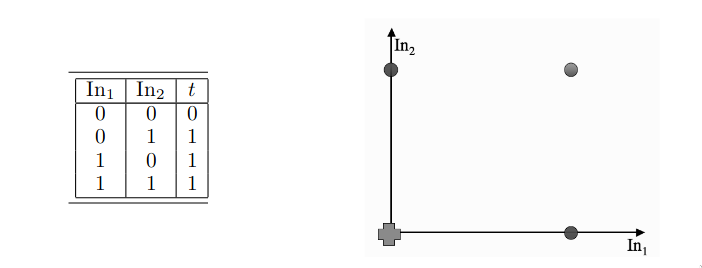
\includegraphics[scale=0.45]{Linn/OR_gate.png}
    \caption{The truth table and plot of the OR gate}
    \label{fig:or_gate}
\end{figure}

\begin{figure}
    \centering
    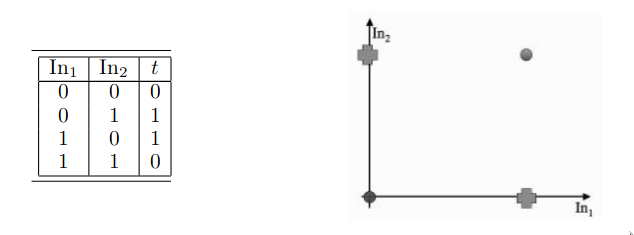
\includegraphics[scale=0.5]{Linn/XOR_gate.png}
    \caption{The truth table and plot of the XOR gate}
    \label{fig:xor_gate}
\end{figure}

\begin{figure}
    \centering
    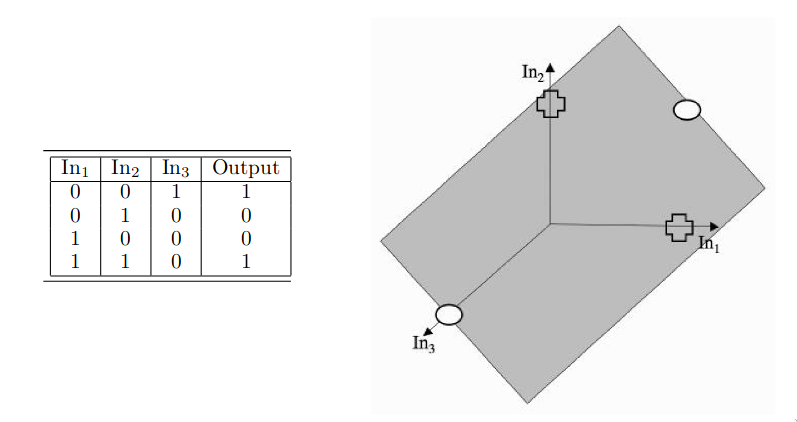
\includegraphics[scale=0.5]{Linn/transform.png}
    \caption{A decision boundary (the shaded plane) solving the XOR problem in 3D with the crosses below the surface and the circles above it.}
    \label{fig:transform}
\end{figure}

\section{Margin and Support Vectors}
An important idea that SVMs make use of is to identify a way to tell apart a good classifier from a bad one. The way the SVM does that is using the idea of a margin. Consider the following figure \ref{fig:compare} that tries to compare different linear classifiers. If you had to pick one classifier from the three which one would you pick? Even though most people might choose the middle one, it is difficult to justify that choice. 

\begin{figure}
    \centering
    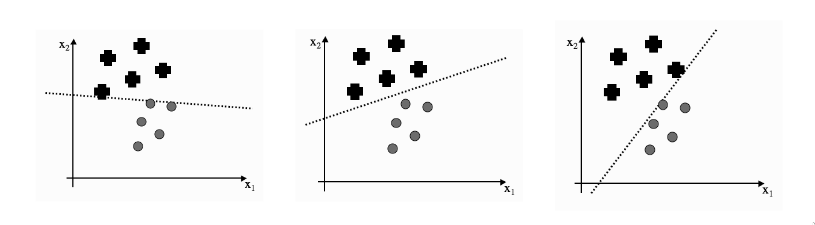
\includegraphics[scale=0.5]{Linn/compare.png}
    \caption{Comparing different linear classifiers. Is there any reason to prefer one over the other?}
    \label{fig:compare}
\end{figure}

The concept of a margin naturally arises while trying to find a criteria for the best classifier. Imagine that we put a ‘no-man’s land’ around the line, so that any point that lies within that region is declared to be too close to the line to be accurately classified, see Figure \ref{fig:margin}.
How large can we make the boundary of this region until we hit actual data points? That particular (half) width is called the margin M. 
The best classifier in Figure \ref{fig:compare} can now be identified as the maximum margin classifier. The data points in each class that lie closest to the  classification line are called support vectors. Two important statements that can be made on the above discussion are: first that the margin should be as large as possible, and second that the support vectors are the most important data points as they are the ones that we might more easily misclassify.


\begin{figure}
    \centering
    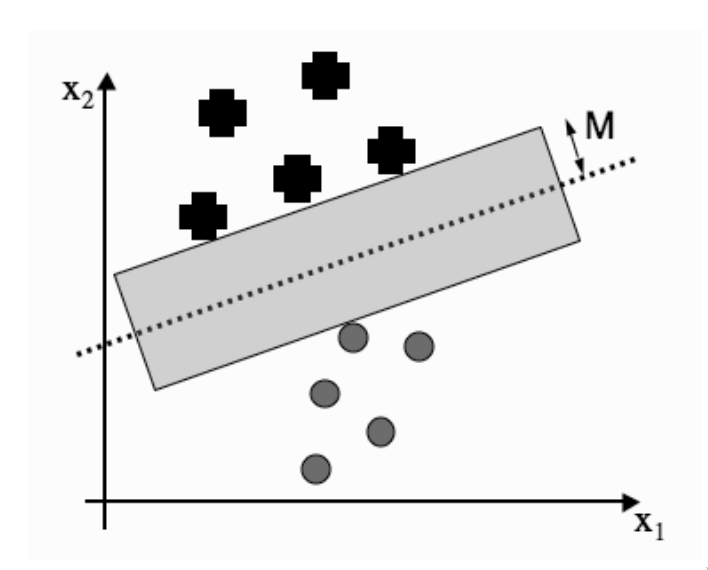
\includegraphics[scale=0.35]{Linn/margin.png}
    \caption{The margin is the largest region that separates the two classes without having any data points in it}
    \label{fig:margin}
\end{figure}

\section{Quadratic Programming}
How do we define a machine learning algorithm that can compute the best classification line based on the concept of the margin and support vectors? 
Similar to the concept of a weight matrix in a neural network we can consider a weight vector \textbf{w} and a bias b that the SVM algorithm tries to learn. Then the actual separating hyperplane is specified by $\mathbf{w}^{T}\mathbf{x}+b = 0$. It can be seen that the margin is given by $1/||w||$. Therefore maximising the margin implies minimizing the weight vector. But if this was the only constraint we could just put $\mathbf{w}=0$ and get it done.  But we also need to make sure that the classifier classifies all the training examples correctly. 
Therefore we need to simultaneously satisfy two problems,  minimize $\mathbf{w}\cdot\mathbf{w}$ subject to some constraints that ensure that the training examples are correctly classified.

The problem described is quadratic and hence convex with linear constraints. Convex functions have a unique minimum, which is fairly easy to see in one dimension, and remains true in any number of dimensions. Such problems can be solved directly and efficiently (in polynomial time). There exists quadratic programming solvers that can solve these equations.


\section{Soft Margin Classifier for Non Linearly Separable Problems}
A non linearly separable dataset introduces an immediate problem.
Now the constraints cannot be satisfied for all of the data points. However this doesn't mean that the algorithm is unusable.
Consider a classifier that misclassifies a point by putting it on the wrong side of the line but very close to it. % Is the classifier placing points or finding lines?
This is obviously better than another one that puts the same points a long way away from the line.
This information can be incorporated into the minimisation criterion. We can add a term such that we are now trying to minimize. $$\mathbf{w}^T\mathbf{w}+ C \times \textrm{(distance of misclassified points from the boundary line)}$$ Here, C is a trade-off parameter that acts as a weight to decide which of the two criteria to favour more. A small C means we prize a large margin over a few errors, while large C means the opposite. This transforms the problem into a soft-margin classifier, since we are allowing for a few mistakes.

\section{Kernel Functions}
In the case of a non linearly separable dataset, even though we can modify the minimisation criteria to account for some misclassification, it wont do much good on it's own. The real reason behind the efficiency of the SVM is what is known as the kernel trick. As mentioned earlier, we can transform the data into a space such that the data becomes linearly separable. We saw earlier that in the case of the XOR gate problem we could make the problem linearly separable by adding a new dimension to the data. But since we cannot invent new data to create extra dimensions, what can be done is create new functions from our existing input features. 
%Knowing something about the data might help in choosing these functions. 
Is there any disadvantages to adding more dimensions to the data in this way? Remember that we need to compute the dot products of our inputs. By increasing the dimensionality of our data we will be increasing the computational expense of our algorithm. 
%This increase might depend  on the number of input features in the original data,  
%However by selecting suitable kernels it can be seen that this dot product can be factorised. 
But in reality, by selecting suitable basis functions for transforming the data we can get away without computing the dot products in this computationaly expensive space and instead just compute a kernel matrix \textbf{K} consisting of the dot products in the low-dimensional space. Any symmetric function that is positive definite (meaning that it enforces positivity on the integral of arbitrary functions) can be used as a kernel. This is a result of Mercer’s theorem. 
Some of the commonly used kernels correspond to basis functions like polynomials of degree n, sigmoid functions, radial basis functions etc. In practice people experiment with the different available functions using a validation set in order to select one that works best. 


    %</note>
    \printbibliography
\end{document}
